
\tikzstyle{startstop} = [rectangle, rounded corners, text centered, draw=black, fill=red!30]
\tikzstyle{process} = [rectangle, text centered, draw=black, fill=orange!30]
\tikzstyle{decision} = [rectangle, text centered, draw=black, fill=green!30]
\tikzstyle{arrow} = [thick,->,>=stealth]

\framebox{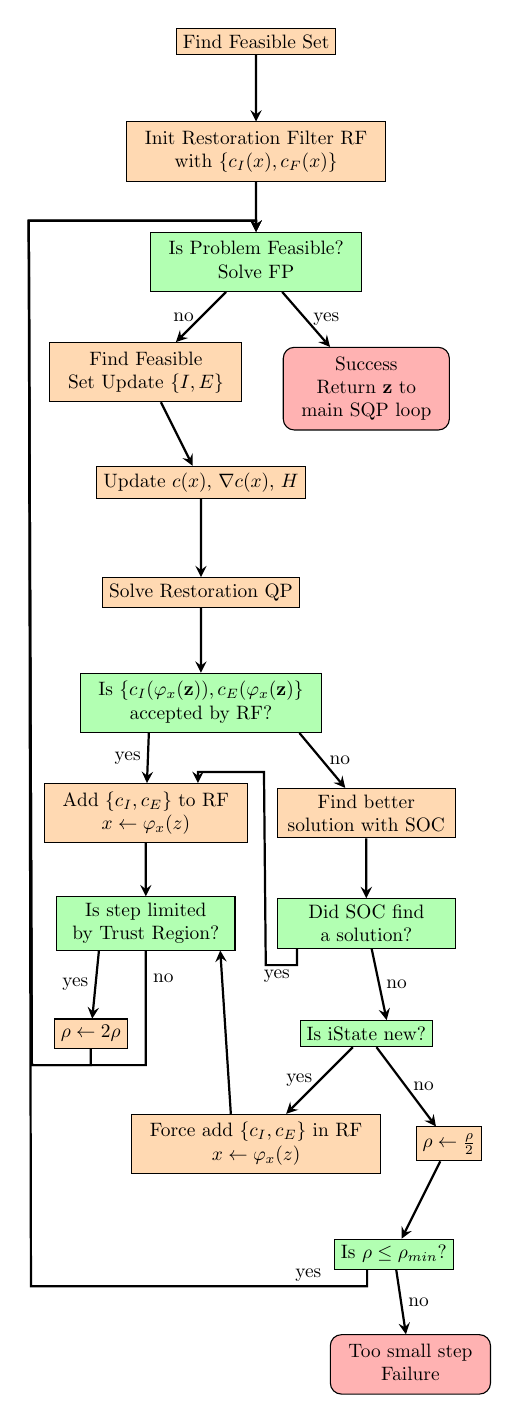
\begin{tikzpicture}[node distance=2cm, scale=0.7, every node/.style={transform shape}]

\node (feasibleSet) [process] {Find Feasible Set};
\node (init) [process, below of=feasibleSet] {\begin{tabular}{c}Init Restoration Filter RF\\with $\{c_I(x),c_F(x)\}$\end{tabular}};
\node (feasibleTest) [decision, below of=init] {\begin{tabular}{c}Is Problem Feasible?\\Solve FP\end{tabular}};
\node (success) [startstop, below of=feasibleTest, xshift=2cm, yshift=-3mm] {\begin{tabular}{c}Success\\Return $\bf z$ to\\main SQP loop\end{tabular} };
\node (findFeasibleSet) [process, below of=feasibleTest, xshift=-2cm] {\begin{tabular}{c} Find Feasible\\ Set Update $\{I,E\}$ \end{tabular}};
\node (update) [process, below of=findFeasibleSet, xshift=1cm] {Update $c(x)$, $\nabla c(x)$, $H$};
\node (QP) [process, below of=update] {Solve Restoration QP};
\node (filterTest) [decision, below of=QP] {\begin{tabular}{c}Is $\{c_I(\varphi_x(\mathbf{z})),c_E(\varphi_x(\mathbf{z})\}$\\accepted by RF?\end{tabular}};
\node (addFilter) [process, below of=filterTest, xshift=-1cm] {\begin{tabular}{c} Add $\{c_I,c_E\}$ to RF\\ $x\leftarrow\varphi_x(z)$\end{tabular}};
\node (stepLimited) [decision, below of=addFilter, text width=3cm] {Is step limited by Trust Region?};
\node (increaseTR) [process, below of=stepLimited, xshift=-1cm] {$\rho\leftarrow 2\rho$};
\node (SOC) [process, below of=filterTest, text width=3cm, xshift=3cm] {Find better solution with SOC};
\node (findSOC) [decision, below of=SOC, text width=3cm] {Did SOC find a solution?};
\node (iStateTest) [decision, below of=findSOC] {Is iState new?};
\node (forceAdd) [process, below of=iStateTest, xshift=-2cm] {\begin{tabular}{c} Force add $\{c_I,c_E\}$ in RF\\ $x\leftarrow\varphi_x(z)$\end{tabular}};
\node (reduceTR) [process, below of=iStateTest, xshift=1.5cm] {$\rho\leftarrow\frac{\rho}{2}$};
\node (tooSmallStep) [decision, below of=reduceTR, xshift=-1cm] {Is $\rho\leq\rho_{min}$?};
\node (fail) [startstop, below of=tooSmallStep, xshift=3mm] {\begin{tabular}{c}Too small step\\
Failure\end{tabular}};

\draw [arrow] (feasibleSet) -- (init);
\draw [arrow] (init) -- (feasibleTest);
\draw [arrow] (feasibleTest) -- node[anchor=west] {yes} (success);
\draw [arrow] (feasibleTest) -- node[anchor=east] {no} (findFeasibleSet);
\draw [arrow] (findFeasibleSet) -- (update);
\draw [arrow] (update) -- (QP);
\draw [arrow] (QP) -- (filterTest);
\draw [arrow] (filterTest.210) -- node[anchor=east] {yes} (addFilter);
\draw [arrow] (filterTest.343) -- node[anchor=west] {no} (SOC);
\draw [arrow] (addFilter) -- (stepLimited);
\draw [arrow] (stepLimited.210) -- node[anchor=east] {yes} (increaseTR);
\draw [arrow] (SOC) -- (findSOC);
\draw [arrow] (findSOC) [xshift=3cm]-- node[anchor=west] {no} (iStateTest);
\draw [arrow] (iStateTest) -- node[anchor=east] {yes} (forceAdd);
\draw [arrow] (iStateTest) -- node[anchor=west] {no} (reduceTR);
\draw [arrow] (reduceTR) -- (tooSmallStep);
\draw [arrow] (tooSmallStep) -- node[anchor=west] {no} (fail);
\draw [arrow] (forceAdd.130) -- (stepLimited.340);

\draw [arrow] (increaseTR) |-([shift={(-4mm,-3mm)}]increaseTR.south west)-- ([shift={(-22mm,2mm)}]feasibleTest.north west)-| (feasibleTest);
\draw [arrow] (stepLimited)  node[anchor=west, yshift=-1cm] {no} |-([shift={(-4mm,-3mm)}]increaseTR.south west)-- ([shift={(-22mm,2mm)}]feasibleTest.north west)-| (feasibleTest);
\draw [arrow] (tooSmallStep.210) node[anchor=east, shift={(-7mm,-1mm)}] {yes} |-([shift={(-55mm,-3mm)}]tooSmallStep.south west)-- ([shift={(-22mm,2mm)}]feasibleTest.north west)-| (feasibleTest);
\draw [arrow] (findSOC.200)  node[anchor=east, yshift=-5mm] {yes} |-([shift={(-2mm,-3mm)}]findSOC.south west) [xshift=1cm]-- ([shift={(3mm,2mm)}]addFilter.north east)-| (addFilter.30);

\end{tikzpicture}
}
